\documentclass{article}
% \pdfplotsset{compat=1.18}
\usepackage[utf8]{inputenc}
\usepackage{bbm} 
\usepackage{tabularx}
\usepackage{amsopn}
\usepackage{amsmath}
\usepackage{amsfonts}
\usepackage{hyperref}
\usepackage{tikz}
\usepackage{pgfplots}

\usepackage{bm}
\title{%
   Homework 2 \\
  \large Fondations of Machine Learning \\}
\author{Xiang Pan (xp2030)}

\begin{document}


\maketitle
\section*{VC Dimension}
\section{}
\subsection*{(a)}
Show that there exists a set of $n+1$ points in $\mathbb{R}^{n}$ that can be shattered by $\mathcal{B}_{n}$. Conclude that VCdim $\left(\mathcal{B}_{n}\right) \geq n+1$


Set condition: We have n+1 points can determine a unique ball in $\mathbb{R}^{n}$, and we have the ball center c, radius r.

For those negative points $p_n \in P_{N}$, we have the radius vector from $p_n$ to c, thus we can constuct the new $p_n' = p_n + \delta(c-p_n)$, $\delta>0$. $p_n' \in P_N'$, $P_N'$ is the set of $p_n'$.

 Thus we can constuct a new ball with new n+1 points set ${P_N'} \bigcup {P_P}$. For the new ball B (c', r'), the negative points distance $r>r'$, the positive points $r'\leq r'$. Thus B (c', r') can shatter n+1 points in $\mathbb{R}^{n}$.

To prove $r > r'$, the B (c,r) and B (c',r') are joint, since $P_P$ are in the B (c,r) and B (c',r'). Note that, $P_N'$ are strictly inside B (c,r), it is easy to check that $P_N$ are strictly outside B (c',r').

There exists a set of (n+1) points in $R^n$ that can be shattered by B(n). We can conclude that VCdim $\left(\mathcal{B}_{n}\right) \geq n+1$.

\subsection*{(b)}

Let $B(c, r)$ be the ball of radius $r$ centered at $c \in \mathbb{R}^{n}$. Then $x \in B(c, r)$

\begin{equation}
    \left\| x - c \right\|^2 \leq r
\end{equation}


\begin{equation}
    \sum_{i=1}^{n}\left\|x_{i}\right\|^{2}-2 \sum_{i=1}^{n} c_{i} x_{i}+\sum_{i=1}^{n} c_{i}^{2}-r \leq 0
\end{equation}

We can find a hyperplane $h$ that is orthogonal to $B(c, r)$ and $x$ is in $B(c, r)$ if $h \cdot x' + b \leq 0$.

\begin{align}
    h =
    \begin{bmatrix}
        1,       \\
        -2c_{1}, \\
        -2c_{2}, \\
        \cdot    \\
        -2c_{n}  \\
    \end{bmatrix}
\end{align}


\begin{align}
    x' =
    \begin{bmatrix}
        \sum_{i=1}^{n} {\|x_{i}\|}^2 \\
        x_{1}                        \\
        x_{2}                        \\
        \cdot                        \\
        x_{n}                        \\
    \end{bmatrix}
\end{align}


\begin{align}
    b = \sum c_{i}^{2} - r
\end{align}

The VC dimension of $B(c, r)$ is at most as the same as the VC dimension of hyperplane $R^{n+1}$, which is n+2.


\subsection*{(c)}
Show that VCdim$\left(\mathcal{B}_{2}\right)=3$.

We have already know that

\begin{align}
    3 \leq \left(\mathcal{B}_{2}\right) \leq 4
\end{align}

But for four points, we can use three points $y_1=1, y_2=1, y_3=1$ to uniquely determine a ball $b_0$ in $\mathbb{R}^{2}$, we can make the fourth point within the ball, and the fourth point is the center of the ball, and the $y_4 = -1$. Any ball can cover $p1, p2, p3$ must cover the minimal ball $b_0$, thus $p4$ must within any ball can cover $p1, p2, p3$. The VC dimension is at most 3.

This case can not find a ball to shatter it.

Thus we have VCdim $\left(\mathcal{B}_{2}\right) = 3$

\section*{Maximum Margin Multiple Kernel}
\section*{1}
\subsection*{(a)}

\begin{equation}
    \widehat{\mathcal{M}}_{q}=\left\{\boldsymbol{\mu}: \boldsymbol{\mu} \in \Delta_{q}, \widehat{\gamma}_{K_{\mu}} \geq \gamma_{0}\right\}
\end{equation}

$\Delta_q$ is the set of $\mu$,

\begin{equation}
    \Delta_{q}=\left\{\boldsymbol{\mu}: \boldsymbol{\mu} \geq 0,\|\boldsymbol{\mu}\|_{q}=1\right\} \text { with } q \geq 1
\end{equation}

K is the combined kernel function, $\mu$ is the weight for each kernel component,

\begin{equation}
    K = \sum_{k=1}^{p} \mu_{k} K_{k}
\end{equation}

To explain $\gamma$, we need to show where the $\gamma_0$ from.

From the paper,
\begin{equation}
    \max _{\boldsymbol{\mu} \in \Delta_{q}} \sum_{i=1}^{m} \min _{y \neq y_{i}} \boldsymbol{\mu} \cdot \boldsymbol{\eta}\left(x_{i}, y_{i}, y\right)
\end{equation}

which equals to

\begin{equation}
    \max _{\boldsymbol{\mu} \in \Delta_{q}} \frac{1}{m} \sum_{i=1}^{m} \min _{y \neq y_{i}} \boldsymbol{\mu} \cdot \boldsymbol{\eta}\left(x_{i}, y_{i}, y\right)
\end{equation}.

Converting the optimization to convex optimization, we have

\begin{equation}
    \max _{\substack{\mu \in \Delta_{q} \\ \gamma}} \sum_{i=1}^{m} \gamma_{i} \text { s.t. } \forall i \in[1, m], \forall y \neq y_{i}, \boldsymbol{\mu} \cdot \boldsymbol{\eta}\left(x_{i}, y_{i}, y\right) \geq \gamma_{i}
    \label{eq:max_margin_convex}
\end{equation}


We can directly solve the optimization problem, however we can convert it to a minimization problem with constraint $\widehat{\gamma}_{K_{\boldsymbol{\mu}}} \geq \gamma_{0}$.

\begin{equation}
    \widehat{\gamma}_{K_{\mu}}=\frac{1}{m} \sum_{i=1}^{m} \min _{y \neq y_{i}} \boldsymbol{\mu} \cdot \boldsymbol{\eta}\left(x_{i}, y_{i}, y\right)
\end{equation}

For $\gamma_0$, setting it equal to the maximum feasible value will guarantee that the selected $\bm{\mu}$ is also give us the solution as\eqref{eq:max_margin_convex}.

\subsection*{(b)}

\begin{equation}
    \begin{aligned}
        \min _{\boldsymbol{\mu} \in \widehat{\mathcal{M}}_{q}} \min _{\mathbf{w}, \boldsymbol{\xi}} & \frac{1}{2} \sum_{y=1}^{c} \sum_{k=1}^{p} \frac{\left\|\mathbf{w}_{y, k}\right\|^{2}}{\mu_{k}}+C \sum_{i=1}^{m} \xi_{i}, \\
        \text{subject to: }                                                                         & \forall i \in[1, m], \xi_{i} \geq 0, \forall y \neq y_{i}                                                                \\
                                                                                                    & \xi_{i} \geq 1-\left(\mathbf{w}_{y_{i}} \cdot \Phi\left(x_{i}\right)-\mathbf{w}_{y} \cdot \Phi\left(x_{i}\right)\right)
    \end{aligned}
\end{equation}

We can trasnform the optimization problem to,

\begin{equation}
    \begin{aligned}
        \min _{\boldsymbol{\mu} \in \widehat{\mathcal{M}}_{q}} \min _{\mathbf{w}, \boldsymbol{\xi}}
         & \beta  \frac{1}{2}  \sum_{y=1}^{c} \left\|\mathbf{w}_{y} \cdot \frac{1}{\sqrt{\bm{\mu}}}\right\|^{2}+\sum_{i=1}^{m} \xi_{i},                    \\
        \text{subject to: }
         & \forall i \in[1, m], \xi_{i} \geq 0,                                                                                                            \\
         & \left(\mathbf{w}_{y_{i}} \cdot \Phi\left(x_{i}\right)-\mathbf{w}_{y} \cdot \Phi\left(x_{i}\right)\right) + \delta_{y_i, y} - 1 + \xi_{i} \geq 0
    \end{aligned}
\end{equation}

\begin{equation}
    \beta = \frac{1}{C}
\end{equation}


$w \in R^{m \times c}$

$\delta_{y_i, y}$ is the indicator function, if $\delta_{y_i, y} = 1$ if $y_i = y$, otherwise it is 0.

\begin{align}
    \begin{aligned}
        \mathcal{L}(\mathbf{w}, \boldsymbol{\xi}, \bm{\alpha})
         & = \beta \frac{1}{2}  \sum_{y=1}^{c} {\left\|\mathbf{w}_{y} \cdot \frac{1}{\sqrt{\bm{\mu}}} \right\|^{2}}
        + \sum_{i=1}^{m} \xi_{i}
        - \sum_{i, y} \alpha_{i, y}\left(\mathbf{w}_{y_{i}} \cdot \Phi\left(x_{i}\right)-\mathbf{w}_{y} \cdot \Phi\left(x_{i}\right)\right) + \delta_{y_i, y} - 1 + \xi_{i}
    \end{aligned}
\end{align}

Then we can get the KKT,

\begin{equation}
    \frac{\partial}{\partial \xi_{i}} \mathcal{L}=1- \sum_{y} \alpha_{i, y}=0 \quad \Rightarrow \quad \sum_{y} \alpha_{i, y} = 1
    \label{eq:2b_xi}
\end{equation}


\begin{equation}
    \begin{aligned}
        \frac{\partial}{\partial \bm{w}_{y}} \mathcal{L} & =
        \beta \bm{w}_{y} \cdot \frac{1}{\bm{\mu}} + \sum_{i} \alpha_{i, y} \Phi({x}_{i})-\sum_{i, y_{i}=y} \underbrace{\left(\sum_{q} \alpha_{i, q}\right)}_{=1} \Phi({x}_{i})          \\
                                                         & =\beta \bm{w}_{y} \cdot \frac{1}{\bm{\mu}} + \sum_{i} \alpha_{i, y} \Phi({x}_{i})- \sum_{i} \delta_{y_{i} y} \Phi({x}_{i})=0
    \end{aligned}
\end{equation}

\begin{equation}
    \bm{w}_{y}=\beta^{-1} \left[\sum_{i}\left(\delta_{y_{i}, y}-\alpha_{i, y}\right) \Phi({x}_{i})\right] \cdot \bm{\mu}
    \label{eq:2b_w}
\end{equation}


By using the KKT\eqref{eq:2b_xi},
\begin{align}
    \begin{aligned}
        \mathcal{L}(\mathbf{w}, \boldsymbol{\xi}, \bm{\alpha})
         & = \beta \frac{1}{2}  \sum_{y=1}^{c} {\left\|\mathbf{w}_{y} \cdot \frac{1}{\sqrt{\bm{\mu}}} \right\|^{2}}
        + \sum_{i=1}^{m} \xi_{i}
        - \sum_{i, y} \alpha_{i, y}\left(\mathbf{w}_{y_{i}} \cdot \Phi\left(x_{i}\right)-\mathbf{w}_{y} \cdot \Phi\left(x_{i}\right)\right) + \delta_{y_i, y} - 1 + \xi_{i}                                             \\
         & = \beta \frac{1}{2}  \sum_{y=1}^{c} {\left\|\mathbf{w}_{y} \cdot \frac{1}{\sqrt{\bm{\mu}}} \right\|^{2}} + \sum_{i=1}^{m} \xi_{i} - \sum_{i, y} \alpha_{i, y} \xi_{i} + \sum_{i, y} \alpha_{i, y} \delta_{y_i, y}
        - \sum_{i, y} \alpha_{i, y} \left(\mathbf{w}_{y_{i}} \cdot \Phi\left(x_{i}\right)-\mathbf{w}_{y} \cdot \Phi\left(x_{i}\right)\right)                                                                            \\
         & = \beta \frac{1}{2}  \sum_{y=1}^{c} {\left\|\mathbf{w}_{y} \cdot \frac{1}{\sqrt{\bm{\mu}}} \right\|^{2}}
        + \sum_{i=1}^{m} \xi_{i} - \sum_{i} \xi_i \underbrace{\sum_{y} \alpha_{i, y}}_{=1} + \sum_{i, y} \alpha_{i, y} \delta_{y_i, y} \\
        &  - \sum_{i, y} \alpha_{i, y} \left(\mathbf{w}_{y_{i}} \cdot \Phi\left(x_{i}\right)-\mathbf{w}_{y} \cdot \Phi\left(x_{i}\right)\right)                                                                            \\
         & =
        \underbrace{\frac{1}{2} \beta  \sum_{y=1}^{c} {\left\|\mathbf{w}_{y} \cdot \frac{1}{\sqrt{\bm{\mu}}} \right\|^{2}}}_{=P1}
        + \underbrace{\sum_{i, y} \alpha_{i, y} \delta_{y_i, y}}_{=P2}
        + \underbrace{\sum_{i, y} \alpha_{i, y} \left(\mathbf{w}_{y} \cdot \Phi\left(x_{i}\right) \right) }_{=P3}
        - \underbrace{\sum_{i, y} \alpha_{i, y} \left(\mathbf{w}_{y_{i}} \cdot \Phi\left(x_{i}\right)\right)}_{=P4}
    \end{aligned}
\end{align}


\begin{align}
    P3 & = \sum_{i, y} \alpha_{i, y} \left(\mathbf{w}_{y} \cdot \Phi\left(x_{i}\right)\right) \\
       & = \beta^{-1} \sum_{i, y} \alpha_{i, y}
    \left(
    \left[
        \sum_{j}\left(\delta_{y_{j}, y}-\alpha_{j, y}\right) \Phi({x}_{j})
        \right]
    \cdot \bm{\mu} \cdot \Phi\left(x_{i}\right)
    \right)                                                                                   \\
       & = \beta^{-1}\sum_{i, y} \alpha_{i, y} \bm{\mu} \cdot
    \left(
    \sum_{j}\left(\delta_{y_{j}, y}-\alpha_{j, y}\right) \Phi({x}_{j})
    \cdot \Phi\left(x_{i}\right)
    \right)                                                                                   \\
       & =\beta^{-1} \sum_{i, y} \alpha_{i, y} \bm{\mu} \cdot
    \left(
    \sum_{j}\left(\delta_{y_{j}, y}-\alpha_{j, y}\right) K(x_i, x_j)
    \right)                                                                                   \\
       & = \beta^{-1} \sum_{i, j} K(x_i, x_j) \bm{\mu}
    \cdot
    \left(
    \sum_{y} \alpha_{i, y} \left(\delta_{y_{j}, y}-\alpha_{j, y}\right)
    \right)
    % &= C \sum_{i, j} K(x_i, x_j) \bm{\mu}
    % \cdot
    % \left(
    % \sum_{y}  \left(\delta_{y_{j}, y}-\alpha_{j, y}\right)
    % \right)
\end{align}

\begin{align}
    P4 & = \sum_{i, y} \alpha_{i, y} \left(\mathbf{w}_{y_{i}} \cdot \Phi\left(x_{i}\right)\right) \\
       & = \beta^{-1} \sum_{i, y} \alpha_{i, y}
    \left(
    \left[
        \sum_{j}\left(\delta_{y_{j}, y_i}-\alpha_{j, y_i}\right) \Phi({x}_{j})
        \right]
    \cdot \bm{\mu} \cdot \Phi\left(x_{i}\right)
    \right)                                                                                       \\
       & = \beta^{-1} \sum_{i, y} \alpha_{i, y} \bm{\mu} \cdot
    \left(
    \sum_{j}\left(\delta_{y_{j}, y_i}-\alpha_{j, y_i}\right) \Phi({x}_{j})
    \cdot \Phi\left(x_{i}\right)
    \right)                                                                                       \\
       & = \beta^{-1} \sum_{i, y} \alpha_{i, y} \bm{\mu} \cdot
    \left(
    \sum_{j}\left(\delta_{y_{j}, y_i}-\alpha_{j, y_i}\right) K(x_i, x_j)
    \right)                                                                                       \\
       & = \beta^{-1} \sum_{i, j} K(x_i, x_j) \bm{\mu}
    \cdot
    \left(\delta_{y_{j}, y_i}-\alpha_{j, y_i}\right)\
    \underbrace{
        \left(
        \sum_{y} \alpha_{i, y}
        \right)
    }_{=1}                                                                                        \\
       & = \beta^{-1} \sum_{i, j} K(x_i, x_j) \bm{\mu}
    \sum_{y} \delta_{y_{j}, y} (\delta_{y_{j}, y}-\alpha_{j, y})
\end{align}


\begin{align}
    P1 & =\beta \frac{1}{2}  \sum_{y=1}^{c} {\left\|\mathbf{w}_{y} \cdot \frac{1}{\sqrt{\bm{\mu}}} \right\|^{2}}                             \\
       & = \beta\frac{1}{2}  \sum_{y=1}^{c} (\mathbf{w}_{y} \cdot \frac{1}{\sqrt{\bm{\mu}}}) \cdot (\mathbf{w}_{y} \cdot \frac{1}{\sqrt{\bm{\mu}}}) \\
       & = \beta^{-1} \frac{1}{2} \sum_{y=1}^{c}
    \left[\sum_{i}\left(\delta_{y_{i}, y}-\alpha_{i, y}\right) \Phi({x}_{i})\right] \cdot
    \left[\sum_{j}\left(\delta_{y_{j}, y}-\alpha_{j, y}\right) \Phi({x}_{j})\right]                                                   \\
       & = \frac{1}{2} \beta^{-1} \sum_{i,j} K(x_i, x_j) \sum_{y}
    (\delta_{y_i, y}-\alpha_{i, y}) (\delta_{y_j, y}-\alpha_{j, y})
\end{align}

\begin{align}
    P3 - P4
     & = \beta^{-1} \sum_{i, j} K(x_i, x_j) \bm{\mu}
    \sum_{y} \alpha_{i, y} \left(\delta_{y_{j}, y}-\alpha_{j, y}\right) \\
     & -
    \beta^{-1}
    \sum_{i, j} K(x_i, x_j) \bm{\mu}
    \sum_{y} \delta_{y_{j}, y} (\delta_{y_{j}, y}-\alpha_{j, y})        \\
     & = - \beta^{-1} \sum_{i,j} K(x_i, x_j) \sum_{y}
    (\delta_{y_i, y}-\alpha_{i, y}) (\delta_{y_j, y}-\alpha_{j, y})
    % &= - \sum_{i, j} K(x_i, x_j) \bm{\mu}
    % \sum_{y} 
    % (\delta_{y_{j}, y}-\alpha_{j, y})
    % (\delta_{y_{j}, y}-\alpha_{j, y})
\end{align}

\begin{align}
    \begin{aligned}
        \mathcal{L}(\mathbf{w}, \boldsymbol{\xi}, \bm{\alpha})
         & =
        \underbrace{\frac{1}{2}  \sum_{y=1}^{c} {\left\|\mathbf{w}_{y} \cdot \frac{1}{\sqrt{\bm{\mu}}} \right\|^{2}}}_{=P1}
        + \underbrace{\sum_{i, y} \alpha_{i, y} \delta_{y_i, y}}_{=P2}
        + \underbrace{\sum_{i, y} \alpha_{i, y} \left(\mathbf{w}_{y} \cdot \Phi\left(x_{i}\right) \right) }_{=P3}
        - \underbrace{\sum_{i, y} \alpha_{i, y} \left(\mathbf{w}_{y_{i}} \cdot \Phi\left(x_{i}\right)\right)}_{=P4}                                                                                                                   \\
         & = \frac{1}{2} \beta^{-1} \sum_{i,j} K(x_i, x_j) \sum_{y}
        (\delta_{y_i, y}-\alpha_{i, y}) (\delta_{y_j, y}-\alpha_{j, y}) \bm{\mu}                                                                                                                                                      \\                                                                                                                                                              \\
         & -  \beta^{-1} \sum_{i,j} K(x_i, x_j) \sum_{y}
        (\delta_{y_i, y}-\alpha_{i, y}) (\delta_{y_j, y}-\alpha_{j, y}) \bm{\mu}                                                                                                                                                      \\
         & + \sum_{i, y} \alpha_{i, y} \delta_{y_i, y}                                                                                                                                                                                \\
         & = - \frac{1}{2} \beta^{-1} \sum_{i,j} K(x_i, x_j) \sum_{y}
        (\delta_{y_i, y}-\alpha_{i, y}) (\delta_{y_j, y}-\alpha_{j, y}) \bm{\mu}                                                                                                                                                      \\
         & + \sum_{i, y} \alpha_{i, y} \delta_{y_i, y}                                                                                                                                                                                \\
         & = - \frac{1}{2} \beta^{-1} \sum_{i,j} K(x_i, x_j) \sum_{y} (\delta_{y_i, y}-\alpha_{i, y}) (\delta_{y_j, y}-\alpha_{j, y}) \bm{\mu}  + \sum_{i, y} \alpha_{i, y} \delta_{y_i, y}                                           \\
         & = - \frac{C}{2} \sum_{i,j} K(x_i, x_j) \sum_{y} (\delta_{y_i, y}-\alpha_{i, y}) (\delta_{y_j, y}-\alpha_{j, y}) \bm{\mu}  + \sum_{i} \alpha_{i} \cdot \bm{1}_{y_i}            &  & \text{(Using $C = \frac{1}{\beta}$)} \\
    \end{aligned}
\end{align}

\begin{align}
    \bm{w}_{y}&=\beta^{-1} \left[\sum_{i}\left(\delta_{y_{i}, y}-\alpha_{i, y}\right) \Phi({x}_{i})\right] \cdot \bm{\mu} \\
              &=\beta^{-1}\left[\sum_{i: y_{i}=y}\left(1-\alpha_{i, y}\right) \Phi(x_i) + \sum_{i: y_{i} \neq y}\left(-\alpha_{i, y}\right) \Phi({x}_{i})\right] \bm{\mu}
\end{align}

Thus we get the following dual problem,

\begin{equation}
    \begin{aligned}
        \min _{\boldsymbol{\mu} \in \widehat{M}_{q}} \max _{\boldsymbol{\alpha} \in \mathbb{R}^{m \times c}} 
        & - \frac{C}{2} \sum_{i,j} K(x_i, x_j) \sum_{y} (\delta_{y_i, y}-\alpha_{i, y}) (\delta_{y_j, y}-\alpha_{j, y}) \bm{\mu}  + \sum_{i} \alpha_{i} \cdot \bm{1}_{y_i} \\
        \text { subject to: }   & \forall i \in[1, m], \boldsymbol{\alpha}_{i} \geq 0 \wedge \bm{\alpha}_{i} \cdot \mathbf{1}= 1
    \end{aligned}
\end{equation}

$L$ is concave in $\bm{\alpha}$.We define the new dual variable $\boldsymbol{\hat{\alpha}}$ as $\bm{\delta}-\bm{\alpha}$:

\begin{equation}
    \hat{\alpha}_{i, y} = \delta_{y_i, y}-\alpha_{i, y}
\end{equation}

\begin{equation}
    \begin{aligned}
        \min _{\boldsymbol{\mu} \in \widehat{M}_{q}} \max _{\boldsymbol{\hat{\alpha}} \in \mathbb{R}^{m \times c}} & \sum_{i=1}^{m} \boldsymbol{\hat{\alpha}}_{i} \cdot \mathbf{e}_{y_{i}}-\frac{C}{2} \sum_{i, j=1}^{m}\left(\boldsymbol{\hat{\alpha}}_{i} \cdot \boldsymbol{\hat{\alpha}}_{j}\right) \sum_{k=1}^{p} \mu_{k} K_{k}\left(x_{i}, x_{j}\right) \\
        \text { subject to: }                                                                                & \forall i \in[1, m], \boldsymbol{\hat{\alpha}}_{i} \leq \mathbf{e}_{y_{i}} \wedge \boldsymbol{\hat{\alpha}}_{i} \cdot \mathbf{1}=0
    \end{aligned}
\end{equation}






% We can derive the Lagrangian Function as
% \begin{align}
%     \begin{aligned}
%         \mathcal{L}(\mathbf{w}, \boldsymbol{\xi}, \bm{\alpha}, \bm{\beta})
%          & = \frac{1}{2} \sum_{y=1}^{c} \sum_{k=1}^{p} \frac{\left\|\bm{w}_{y, k}\right\|^{2}}{\mu_{k}}
%         + C \sum_{i=1}^{m} \xi_{i}                                                                      \\
%          & - \sum_{i=1}^{m}
%         \sum_{y \neq y_i}
%         \alpha_{i, y}
%         \left(
%         \bm{w}_{y_{i}} \cdot \Phi\left(x_{i}\right)
%         - \bm{w}_{y} \cdot \Phi\left(x_{i}\right)
%         + \xi_{i}
%         - 1
%         \right)
%         - \sum_{i=1}^{m} \beta_{i} \xi_{i}
%     \end{aligned}
% \end{align}

% \begin{align}
%     \begin{aligned}
%         \mathcal{L}(\mathbf{w}, \boldsymbol{\xi}, \bm{\alpha})
%          & = \frac{1}{2} \sum_{y=1}^{c} \sum_{k=1}^{p} \frac{\left\|\bm{w}_{y, k}\right\|^{2}}{\mu_{k}}
%         + C \sum_{i=1}^{m} \xi_{i}                                                                      \\
%          & - \sum_{i=1}^{m}
%         \sum_{y \neq y_i}
%         \alpha_{i, y}
%         \left(
%         \bm{w}_{y_{i}} \cdot \Phi\left(x_{i}\right)
%         + \xi_{i} - 1
%         \right)                                                                                         \\
%          & + \sum_{i=1}^{m}
%         \sum_{y \neq y_i}
%         \alpha_{i, y} \bm{w}_{y} \cdot \Phi\left(x_{i}\right)                                           \\
%          & - \sum_{i=1}^{m} \beta_{i} \xi_{i}
%     \end{aligned}
% \end{align}

% % We define,
% % \begin{equation}
% %     W' = 
% % \end{equation}



% m is the dataset size, c is the number of classes, p is the number of kernel components.

% Using KKT,
% \begin{align}
%     \begin{aligned}
%         \nabla_{\bm{w}_{y, k}} \mathcal{L} =
%         \frac{\bm{w}_{y, k}}{\mu_k} -
%         \sum_{i: y_i = y} \sum_{y' \neq y} \alpha_{i, y'} \Phi_k(x_i)
%         +\sum_{i: y_i \neq y}   \alpha_{i, y} \Phi_k(x_i) = 0
%     \end{aligned} \\
%     \quad \Longrightarrow \quad
%     w_{y, k} =
%     \mu_k
%     \left(
%     \sum_{i: y_i = y} \sum_{y' \neq y} \alpha_{i, y'} \Phi_k(x_i) -\sum_{i: y_i \neq y}  \alpha_{i, y} \Phi_k(x_i)
%     \right)                                                      \\
%     \mu_k
%     \left(
%     \sum_{i: y_i = y} \Phi_k(x_i)
%     \sum_{y' \neq y} \alpha_{i, y'}  -\sum_{i: y_i \neq y}  \alpha_{i, y} \Phi_k(x_i)
%     \right)                                                      \\
%     \mu_k
%     \left(
%     \sum_{i: y_i = y} \Phi_k(x_i)
%     ((\sum_{y''} \alpha_{i, y''}) - \alpha_{i, y}))
%     -\sum_{i: y_i \neq y}  \alpha_{i, y} \Phi_k(x_i)
%     \right)                                                      \\
%     \mu_k
%     \left(
%     \sum_{i: y_i = y} \Phi_k(x_i)
%     \sum_{y''} \alpha_{i, y''}
%     -\sum_{i: y_i = y}   \alpha_{i, y} \Phi_k(x_i)
%     -\sum_{i: y_i \neq y}  \alpha_{i, y} \Phi_k(x_i)
%     \right)                                                      \\
%     \mu_k
%     \left(
%     \sum_{i: y_i = y} \Phi_k(x_i)
%     \sum_{y''} \alpha_{i, y''}
%     -\sum_{i=1}^{m}   \alpha_{i, y} \Phi_k(x_i)
%     \right)
% \end{align}


% \begin{equation}
%     \nabla_{\xi_{i}} \mathcal{L}=C- \sum_{y \neq y_i} \alpha_{i,y}- \beta_{i}=0
%     \quad \Longrightarrow \quad
%     \sum_{y \neq y_i}\alpha_{i, y}+\beta_{i}=C
% \end{equation}

% \begin{equation}
%     \begin{aligned}
%         \forall {i} \wedge \{y \neq y_i\},
%         \alpha_{i, y}
%         \left(
%         \bm{w}_{y_{i}} \cdot \Phi\left(x_{i}\right)
%         - \bm{w}_{y} \cdot \Phi\left(x_{i}\right)
%         + \xi_{i}
%         - 1
%         \right) = 0 \\
%         \quad \Longrightarrow \quad
%         \alpha_{i, y} = 0 \vee
%         \left[
%             \left(
%             \bm{w}_{y_{i}} \cdot \Phi\left(x_{i}\right)
%             - \bm{w}_{y} \cdot \Phi\left(x_{i}\right)
%             \right)
%             = 1 - \xi_{i}
%             \right]
%     \end{aligned}
% \end{equation}

% \begin{equation}
%     \forall i, \beta_{i} \xi_{i}=0 \quad \Longrightarrow \quad \beta_{i}=0 \vee \xi_{i}=0
% \end{equation}



% Using the KKT condition,
% \begin{align}
%     \begin{aligned}
%         \mathcal{L}(\mathbf{w}, \boldsymbol{\xi}, \bm{\alpha}, \bm{\beta})
%          & = \frac{1}{2} \sum_{y=1}^{c} \sum_{k=1}^{p} \frac{\left\|\bm{w}_{y, k}\right\|^{2}}{\mu_{k}}
%         + C \sum_{i=1}^{m} \xi_{i}                                                                      \\
%          & - \sum_{i=1}^{m}
%         \sum_{y \neq y_i}
%         \alpha_{i, y}
%         \left(
%         \bm{w}_{y_{i}} \cdot \Phi\left(x_{i}\right)
%         - \bm{w}_{y} \cdot \Phi\left(x_{i}\right)
%         + \xi_{i}
%         - 1
%         \right)
%         - \sum_{i=1}^{m} \beta_{i} \xi_{i}
%     \end{aligned}
% \end{align}


% \begin{equation}
%     \frac{1}{2} \sum_{y=1}^{c} \sum_{k=1}^{p} \frac{\left\|\mathbf{w}_{y, k}\right\|^{2}}{\mu_{k}}+C \sum_{i=1}^{m} \xi_{i} - \sum_{i=1}^{m}
%     \sum_{y \neq y_i}
%     \alpha_{i, y}
%     \left(
%     \bm{w}_{y_{i}} \cdot \Phi\left(x_{i}\right)
%     - \bm{w}_{y} \cdot \Phi\left(x_{i}\right)
%     + \xi_{i}
%     - 1
%     \right)
%     - \sum_{i=1}^{m} \beta_{i} \xi_{i}
% \end{equation}

% \begin{equation}
%     \frac{1}{2} \sum_{y=1}^{c} \sum_{k=1}^{p} \frac{\left\|\mathbf{w}_{y, k}\right\|^{2}}{\mu_{k}}+C \sum_{i=1}^{m} \xi_{i} -
%     \sum_{i=1}^{m}
%     \sum_{y \neq y_i}
%     \alpha_{i, y}
%     \sum_{k=1}^{p}
%     \left(
%     \bm{w}_{y_{i}, k} \cdot \Phi_k \left(x_{i}\right)
%     - \bm{w}_{y, k} \cdot \Phi_k \left(x_{i}\right)
%     \right)
%     -
%     \sum_{i=1}^{m}
%     \sum_{y \neq y_i}
%     \alpha_{i, y}{
%         (\xi_{i}
%         - 1)
%     }
%     - \sum_{i=1}^{m} \beta_{i} \xi_{i}
% \end{equation}

% % \begin{equation}
% %     \frac{1}{2} \sum_{y=1}^{c} \sum_{k=1}^{p} \frac{\left\|\mathbf{w}_{y, k}\right\|^{2}}{\mu_{k}}
% %      - 
% %     \sum_{i=1}^{m} 
% %     \sum_{y \neq y_i}
% %      \alpha_{i, y}
% %     \sum_{k=1}^{p}
% %      \left(
% %          (\bm{w}_{y_{i}, k} \cdot \Phi_k \left(x_{i}\right)
% %          - \bm{w}_{y, k} \cdot \Phi_k \left(x_{i}\right)) - 1
% %      \right)
% % \end{equation}


% \begin{equation}
%     \sum_{i=1}^{m} \sum_{y \neq y_i}
%     \alpha_{i, y}
%     +
%     \frac{1}{2} \sum_{y=1}^{c} \sum_{k=1}^{p} \frac{\left\|\mathbf{w}_{y, k}\right\|^{2}}{\mu_{k}}
%     -
%     \sum_{i=1}^{m}
%     \sum_{y \neq y_i}
%     \alpha_{i, y}
%     \sum_{k=1}^{p}
%     \left(
%     (\bm{w}_{y_{i}, k} \cdot \Phi_k \left(x_{i}\right)
%     - \bm{w}_{y, k} \cdot \Phi_k \left(x_{i}\right))
%     \right)
% \end{equation}


% % \begin{equation}
% %     w_{y,k} = \mu_k
% %     \left(
% %         \sum_{i: y_i = y} \Phi_k(x_i) 
% %         \sum_{y''} \alpha_{i, y''}
% %         -\sum_{i=1}^{m}   \alpha_{i, y} \Phi_k(x_i)
% %     \right) 
% % \end{equation}

% % \begin{equation}
% %     \frac{1}{2}
% %     \sum_{y=1}^{c} \sum_{k=1}^{p} \mu_k     \left(
% %         \sum_{i: y_i = y} \Phi_k(x_i) 
% %         \sum_{y''} \alpha_{i, y''}
% %         -\sum_{i=1}^{m}   \alpha_{i, y} \Phi_k(x_i)
% %     \right)^2
% % \end{equation}

% % \begin{equation}
% %     \frac{1}{2}
% %     \sum_{k=1}^{p} \sum_{y=1}^{c}  \mu_k     \left(
% %         \sum_{i: y_i = y} \Phi_k(x_i) 
% %         \sum_{y''} \alpha_{i, y''}
% %         -\sum_{i=1}^{m}   \alpha_{i, y} \Phi_k(x_i)
% %     \right)^2
% % \end{equation}

% \begin{equation}
%     \begin{aligned}
%          & \min _{\boldsymbol{\mu} \in \bar{M}_{q}} \max _{\boldsymbol{\alpha} \in \mathbb{R}^{m \times c}} \sum_{i=1}^{m} \boldsymbol{\alpha}_{i} \cdot \mathbf{e}_{y_{i}}-\frac{C}{2} \sum_{i, j=1}^{m}\left(\boldsymbol{\alpha}_{i} \cdot \boldsymbol{\alpha}_{j}\right) \sum_{k=1}^{p} \mu_{k} K_{k}\left(x_{i}, x_{j}\right) \\
%          & \text { subject to: } \forall i \in[1, m], \boldsymbol{\alpha}_{i} \leq \mathbf{e}_{y_{i}} \wedge \boldsymbol{\alpha}_{i} \cdot \mathbf{1}=0
%     \end{aligned}
% \end{equation}

\newpage

\section*{SVMs hand-on}

The code is available at \url{https://github.com/Xiang-Pan/NYU_FML/blob/master/HW2/c.ipynb}.

\section*{3}
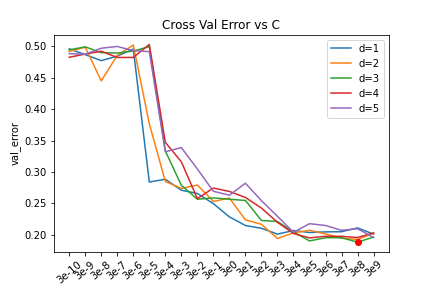
\includegraphics[width=\textwidth]{images/C3_cross_val_error_vs_d.png}

The red point is the optimizal combination. The best pair is d = 3, and C = 6561.0. (C*, d*) = (6561.0, 3). The error is 18.8197\%.


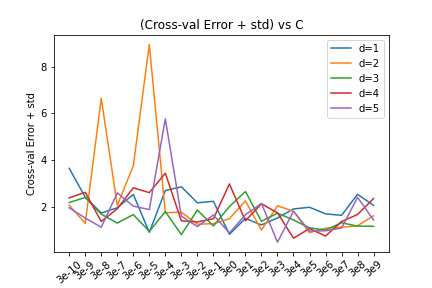
\includegraphics[width=\textwidth]{./images/C3_cross_val_error_plus_std_vs_d.png}


\section*{4}

$(C^*, d^*) = (6561.0, 3)$.

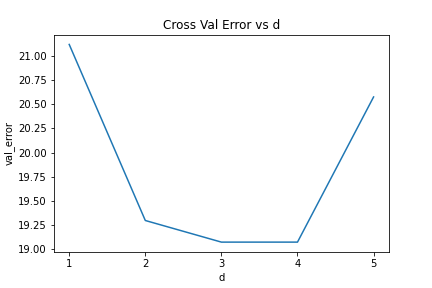
\includegraphics[width=\textwidth]{./images/C4_cross_val_error_vs_d.png}

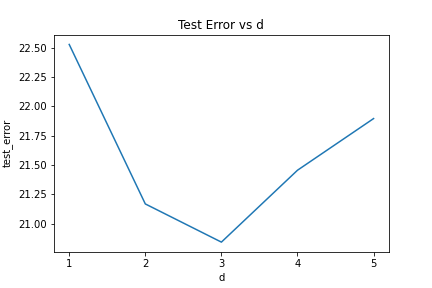
\includegraphics[width=\textwidth]{./images/C4_test_error_vs_d.png}

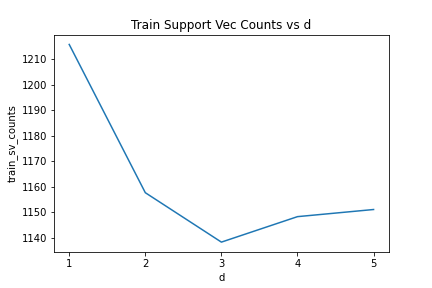
\includegraphics[width=\textwidth]{./images/C4_train_sv_counts.png}

\newpage

\section*{5}

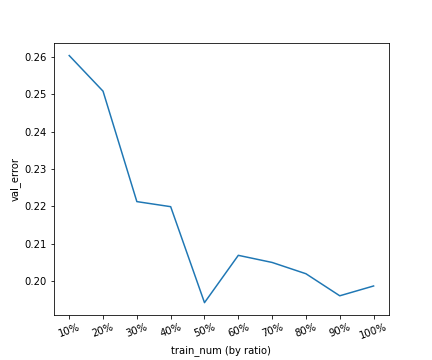
\includegraphics[width=\textwidth]{./images/C5_val_error_vs_train_num.png}

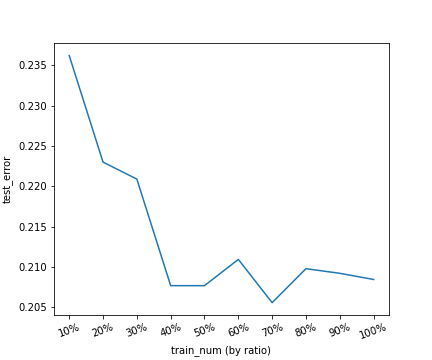
\includegraphics[width=\textwidth]{./images/C5_test_error_vs_train_num.png}

\section*{6}
\subsection*{(a)}
\begin{equation}
    \begin{aligned}
        \min _{\boldsymbol{\alpha}, b, \boldsymbol{\xi}} \frac{1}{2} \sum_{i=1}^{m}\left|\alpha_{i}\right|+C \sum_{i=1}^{m} \xi_{i}                               \\
        \text { subject to } y_{i}\left(\sum_{j=1}^{m} \alpha_{j} y_{j} K\left(\boldsymbol{x}_{i}, \boldsymbol{x}_{j}\right)+b\right) \geq 1-\xi_{i}, i \in[1, m] \\
        \xi_{i}, \alpha_{i} \geq 0, i \in[1, m] .
    \end{aligned}
\end{equation}

We have the Lagrangian function:

\begin{align}
    \mathcal{L}(\bm{\alpha}, b, \bm{\xi}, \bm{\delta}, \bm{\beta}, \bm{\gamma})
     & =\frac{1}{2} \sum_{i=1}^{m}\left|\alpha_{i}\right|
    + C \sum_{i=1}^{m} {\xi}_{i}
    - \sum_{i=1}^{m}
    \delta_{i}
    \left(
    y_{i}\left(\sum_{j=1}^{m} \alpha_{j} y_{j} K\left(\boldsymbol{x}_{i}, \boldsymbol{x}_{j}\right)+b\right) - 1 + \xi_{i}
    \right)                                               \\
     & - \sum_{i=1}^{m} \beta_{i} \xi_{i}
    - \sum_{i=1}^{m} \gamma_{i} \alpha_{i}
    % &= \frac{1}{2} |\bm{\alpha}|
    % + C \sum_{i=1}^{m} \bm{\xi}_{i}
    % - \sum_{i=1}^{m}
    % \delta_{i}
    % \left(
    %     y_{i}\left(\sum_{j=1}^{m} \alpha_{j} y_{j} K\left(\boldsymbol{x}_{i}, \boldsymbol{x}_{j}\right)+b\right) - 1 + \xi_{i}
    % \right)
\end{align}


The KKT conditions are obtained by setting the gradient of the Lagrangian with respect to the primal variables $\bm{\alpha}$, $b$, $\bm{\xi}$ to zero:

\begin{equation}
    \begin{aligned}
        \nabla_{\alpha_{j}} \mathcal{L} =
        \frac{1}{2} sign(\alpha_{j})
        -
        \sum_{i=1}^{m}
        \delta_{i}
        y_{i}
        \left(
        y_{j} K\left(\boldsymbol{x}_{i}, \boldsymbol{x}_{j}\right)
        \right)
        - \gamma_{j}
        = 0 \\
        \quad \Longrightarrow \quad
        \frac{1}{2} sign(\alpha_{j}) =
        \sum_{i=1}^{m}
        \delta_{i}
        y_{i}
        y_{j} K\left(\boldsymbol{x}_{i}, \boldsymbol{x}_{j}\right)
        + \gamma_{j}
    \end{aligned}
    \label{eq:KKT}
\end{equation}\

\begin{equation}
    \nabla_{b} \mathcal{L}=
    -\sum_{i=1}^{m} \delta_{i} y_{i}=0
    \quad \Longrightarrow \quad \sum_{i=1}^{m} \delta_{i} y_{i}=0
\end{equation}

\begin{eqnarray}
    \ = - \frac{C}{2} \sum_{i,j} K(x_i, x_j) \sum_{y} (\delta_{y_i, y}-\alpha_{i, y}) (\delta_{y_j, y}-\alpha_{j, y}) \bm{\mu}  + \sum_{i, y} \alpha_{i, y} \delta_{y_i, y} 
\end{eqnarray}

\begin{equation}
    \nabla_{\xi_{i}} \mathcal{L}=C-\delta_{i}-\beta_{i}=0 \quad \Longrightarrow \quad \delta_{i}+\beta_{i}=C
\end{equation}

\begin{equation}
    \begin{aligned}
        \forall i, \delta_{i}
        \left(
        y_{i}\left(\sum_{j=1}^{m} \alpha_{j} y_{j} K\left(\boldsymbol{x}_{i}, \boldsymbol{x}_{j}\right)+b\right) - 1 + \xi_{i}
        \right)
        = 0 \\
        \quad \Longrightarrow \quad
        \delta_{i}=0
        \vee
        y_{i}\left(\sum_{j=1}^{m} \alpha_{j} y_{j} K\left(\boldsymbol{x}_{i}, \boldsymbol{x}_{j}\right)+b\right) = 1 - \xi_{i}
    \end{aligned}
    \label{eq:constraint}
\end{equation}


\begin{align}
    \forall i, \beta_{i} \xi_{i} & =0 \quad \Longrightarrow \quad \beta_{i}=0 \vee \xi_{i}=0 \\
                                 & \quad \Leftrightarrow \quad \delta_i = C \vee \xi_{i}=0
\end{align}

To derive the dual form of the constrained optimization, we plug into the Lagrangian the definition of $\bm{\alpha}$ in term of the dual variables \eqref{eq:KKT} and apply the constraint \eqref{eq:constraint}:



\begin{equation}
    \mathcal{L}(\bm{\alpha}, b, \bm{\xi}, \bm{\delta}, \bm{\beta}, \bm{\gamma})
    = \frac{1}{2} \sum_{i=1}^{m}\left|\alpha_{i}\right|
    + C \sum_{i=1}^{m} \bm{\xi}_{i}
    - \sum_{i=1}^{m}
    \delta_{i}
    \left(
    y_{i}\left(\sum_{j=1}^{m} \alpha_{j} y_{j} K\left(\boldsymbol{x}_{i}, \boldsymbol{x}_{j}\right)+b\right) - 1 + \xi_{i}
    \right)
    - \sum_{i=1}^{m} \beta_{i} \xi_{i}
    - \sum_{i=1}^{m} \gamma_{i} \alpha_{i}
\end{equation}

\begin{align}
    \mathcal{L}(\bm{\alpha}, b, \bm{\xi}, \bm{\delta}, \bm{\beta}, \bm{\gamma})
     & = \frac{1}{2} \sum_{j=1}^{m}  sign(\alpha_{j}) \cdot \alpha_{j}
    + \sum_{i=1}^{m}  (\delta_i + \beta_i) \bm{\xi}_{i} \\
    &- \sum_{i=1}^{m}
    \delta_{i}
    \left(
    y_{i}\left(\sum_{j=1}^{m} \alpha_{j} y_{j} K\left(\boldsymbol{x}_{i}, \boldsymbol{x}_{j}\right)+b\right) - 1 + \xi_{i}
    \right)
    - \sum_{i=1}^{m} \gamma_{i} \alpha_{i}                             \\
     & = \frac{1}{2} \sum_{j=1}^{m}  sign(\alpha_{j}) \cdot a_{j}
    - \sum_{i=1}^{m}
    \sum_{j=1}^{m}
    \left( \delta_{i}
    y_{i} \alpha_{j} y_{j} K\left(\boldsymbol{x}_{i}, \boldsymbol{x}_{j}\right)+b \delta_{i}
    y_{i} - \delta_i \right)  - \sum_{1}^{m} \gamma_{i} \alpha_{i}
    \\
     & =
    \sum_{j=1}^{m}
    \left(
    \sum_{i=1}^{m}
    \delta_{i}
    y_{i}
    y_{j} K\left(\boldsymbol{x}_{i}, \boldsymbol{x}_{j}\right)
    + \gamma_{j}\right) \cdot a_{j}
    - \sum_{i=1}^{m}
    \sum_{j=1}^{m}
    \left( \delta_{i}
    y_{i} \alpha_{j} y_{j} K\left(\boldsymbol{x}_{i}, \boldsymbol{x}_{j}\right)+b \delta_{i}
    y_{i} - \delta_i \right)  - \sum_{1}^{m} \gamma_{i} \alpha_{i}
    \\
     & =
    \sum_{j=1}^{m}
    \left(
    \sum_{i=1}^{m}
    \delta_{i}
    y_{i}
    y_{j}  a_{j} K\left(\boldsymbol{x}_{i}, \boldsymbol{x}_{j} \right)
    \right)
    - \sum_{i=1}^{m}
    \sum_{j=1}^{m}
    \left( \delta_{i}
    y_{i} \alpha_{j} y_{j} K\left(\boldsymbol{x}_{i}, \boldsymbol{x}_{j}\right)+b \delta_{i}
    y_{i} - \delta_i \right)
    \\
     & =
    \sum_{i=1}^{m}
    \left(
    \sum_{j=1}^{m}
    \delta_{i}
    y_{i}
    y_{j}  a_{j} K\left(\boldsymbol{x}_{i}, \boldsymbol{x}_{j}\right)
    \right)
    -
    \sum_{i=1}^{m}
    \sum_{j=1}^{m}
    \left( \delta_{i}
    y_{i} \alpha_{j} y_{j} K\left(\boldsymbol{x}_{i}, \boldsymbol{x}_{j}\right)+b \delta_{i}
    y_{i} - \delta_i \right)
    % &= 
    % \sum_{i=1}^{m}
    % \left[
    %     \sum_{j=1}^{m}
    %     \delta_{j}
    %     y_{i}
    %         y_{j} K\left(\boldsymbol{x}_{i}, \boldsymbol{x}_{j}\right)
    %     + \gamma_{j}
    % \right] \alpha_i 
    % - \sum_{i=1}^{m}
    % \delta_{i}
    % y_{i}\left(\sum_{j=1}^{m} \alpha_{j} y_{j} K\left(\boldsymbol{x}_{i}, \boldsymbol{x}_{j}\right)+b - 1 \right) \\
    % &= 
    % \sum_{i=1}^{m}
    % \left[
    %     \sum_{j=1}^{m}
    %     \alpha_i 
    %     \delta_{j}
    %     y_{i}
    %         y_{j} K\left(\boldsymbol{x}_{i}, \boldsymbol{x}_{j}\right)
    % \right] 
    % - \sum_{i=1}^{m}
    % \delta_{i}
    % y_{i}\left(\sum_{j=1}^{m} \alpha_{j} y_{j} K\left(\boldsymbol{x}_{i}, \boldsymbol{x}_{j}\right)+b - 1 \right) \\
    % &= 
    % \sum_{j=1}^{m}
    % \left[
    %     \sum_{i=1}^{m}
    %     \alpha_j 
    %     \delta_{i}
    %     y_{j}
    %         y_{i} K\left(\boldsymbol{x}_{i}, \boldsymbol{x}_{j}\right)
    % \right] 
    % - \sum_{i=1}^{m}
    % \delta_{i}
    % y_{i}\left(\sum_{j=1}^{m} \alpha_{j} y_{j} K\left(\boldsymbol{x}_{i}, \boldsymbol{x}_{j}\right)+b - 1 \right) 
    % \\
    % &= 
    % \sum_{i=1}^{m}
    % \left[
    %     \sum_{j=1}^{m}
    %     \alpha_j 
    %     \delta_{i}
    %     y_{j}
    %         y_{i} K\left(\boldsymbol{x}_{i}, \boldsymbol{x}_{j}\right)
    % \right] 
    % - \sum_{i=1}^{m}
    % \delta_{i}
    % y_{i}\left(\sum_{j=1}^{m} \alpha_{j} y_{j} K\left(\boldsymbol{x}_{i}, \boldsymbol{x}_{j}\right)+b - 1 \right) 
    % \\
    % &= 
    % \sum_{i=1}^{m}
    % y_{i} \delta_{i}
    % \left[
    %     \sum_{j=1}^{m}
    %     \alpha_j 
    %     y_{j}
    %         K\left(\boldsymbol{x}_{i}, \boldsymbol{x}_{j}\right)
    % \right] 
    % - \sum_{i=1}^{m}
    % \delta_{i}
    % y_{i}\left(\sum_{j=1}^{m} \alpha_{j} y_{j} K\left(\boldsymbol{x}_{i}, \boldsymbol{x}_{j}\right)+b - 1 \right) 
    \\
     & =
    -
    \sum_{i=1}^{m}
    b
    \delta_{i} y_i- \delta_i
    \\
     & =
    \sum_{i=1}^{m}
    \delta_i
\end{align}

The dual problem is,

\begin{equation}
    \begin{aligned}
        \min _{\boldsymbol{\delta}} \sum_{i=1}^{m} \delta_{i}                                     \\
        \text { subject to: }
        \forall i: \delta_i = C \vee \xi_{i}=0                                                    \\
        \forall i: \delta_{i}=0
        \vee
        y_{i}\left(\sum_{j=1}^{m} \alpha_{j} y_{j} \Phi(x_i)^T \Phi(x_j)  +b\right) = 1 - \xi_{i} \\
        \forall i: \alpha_{i} \geq 0                                                              \\
        \forall i: \xi_{i} \geq 0                                                                 \\
        % y_{i}\left(\sum_{j=1}^{m} \alpha_{j} y_{j} K\left(\boldsymbol{x}_{i}, \boldsymbol{x}_{j}\right)+b\right) \geq 1-\xi_{i}, i \in[1, m] \\
        % \xi_{i}, \alpha_{i} \geq 0, i \in[1, m] .
    \end{aligned}
\end{equation}




% \begin{align}
%     \frac{1}{2} \sum_{j=1}^{m}  sign(\alpha_{j}) \cdot a_{j}
%     &= \sum_{j=1}^{m}
%     \sum_{i=1}^{m}
%     \left[
%         \delta_{i}
%         \left(
%         y_{i}\left(  y_{j} K\left(\boldsymbol{x}_{i}, \boldsymbol{x}_{j}\right)+b y_i\right) - 1 + \xi_{i}
%         \right)
%     \right]+ \gamma_{j} \alpha_j \\
%     &= \sum_{i=1}^{m} \sum_{j=1}^{m}
%     \left[
%         \delta_{j}
%         \left(
%         y_{j} \left(  y_{i} K\left(\boldsymbol{x}_{i}, \boldsymbol{x}_{j}\right)+b y_j\right) - 1 + \xi_{j}
%         \right)
%     \right] + \gamma_{i} \alpha_i \\
% \end{align}




% \mathcal{L}(\mathbf{w}, b, \boldsymbol{\xi}, \boldsymbol{\alpha}, \boldsymbol{\beta})=\frac{1}{2}\|\mathbf{w}\|^{2}+C \sum_{i=1}^{m} \xi_{i}-\sum_{i=1}^{m} \alpha_{i}\left[y_{i}\left(\mathbf{w} \cdot \mathbf{x}_{i}+b\right)-1+\xi_{i}\right]-\sum_{i=1}^{m} \beta_{i} \xi_{i}


\subsection*{(b)}
Derive the equivalent hinge loss minimization problem
\begin{equation}
    \begin{aligned}
        \min _{\boldsymbol{\alpha}, b, \boldsymbol{\xi}} \frac{1}{2} \sum_{i=1}^{m}\left|\alpha_{i}\right|+C \sum_{i=1}^{m} \xi_{i}                               \\
        \text { subject to } y_{i}\left(\sum_{j=1}^{m} \alpha_{j} y_{j} K\left(\boldsymbol{x}_{i}, \boldsymbol{x}_{j}\right)+b\right) \geq 1-\xi_{i}, i \in[1, m] \\
        \xi_{i}, \alpha_{i} \geq 0, i \in[1, m] .
    \end{aligned}
\end{equation}

The equivalent hinge loss optimization problem is:

\begin{equation}
    \begin{aligned}
        \min _{\boldsymbol{\alpha}, b} \frac{1}{2} \sum_{i=1}^{m}\left|\alpha_{i}\right|+C \sum_{i=1}^{m}
        \left(
        1 - y_i
        \left(
            \sum_{j=1}^{m} \alpha_{j} y_{j} K\left(\boldsymbol{x}_{i}, \boldsymbol{x}_{j}\right)+b
            \right)
        \right)_+
        \\
        \alpha_{i} \geq 0, i \in[1, m] .
    \end{aligned}
\end{equation}

\begin{equation}
    \begin{aligned}
        \min _{\boldsymbol{\alpha}, b} \frac{1}{2} \sum_{i=1}^{m}\left|\alpha_{i}\right|+C \sum_{i=1}^{m}
        \left(
        1 -
        \left(
            \sum_{j=1}^{m}
            \alpha_{j}
            y_i \Phi(x_i)^T y_{j} \Phi(x_j)
            +b y_i
            \right)
        \right)_+
        \\
        \alpha_{i} \geq 0, i \in[1, m] .
    \end{aligned}
\end{equation}

$ \hat{y} =\left(\sum_{j=1}^{m} \alpha_{j} y_{j} K\left(\boldsymbol{x}_{i}, \boldsymbol{x}_{j}\right)+b\right)$ which is obtained by kernel trick, thus the equivalent problem is trying to get a trade-off between the sparsity of $\alpha$ and the error.

\textbf{Comparing to the original svm:}
The original svm is trying to get a trade-off between the max margin and the error, and $\hat{y}$ is from definition $wx+b$.

\subsection*{(c)}

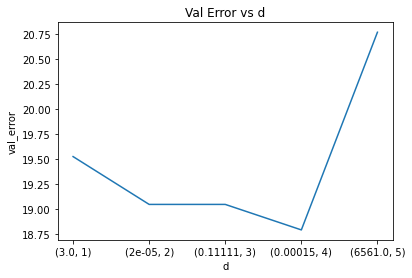
\includegraphics[width=\linewidth]{./images/C6_val_error_vs_d.png}

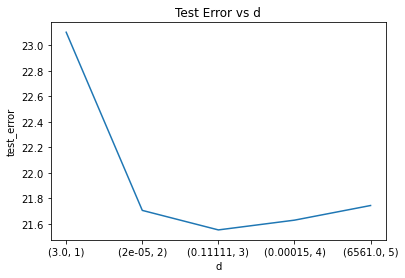
\includegraphics[width=\linewidth]{./images/C6_test_error_vs_d.png}

We use the tuple (C, d) as the x-axis index, d is from 1 to 5, and C is selected based on the best validation error.


\newpage

\bibliographystyle{plain}
\bibliography{main}
\nocite*{}




\end{document}
